% - 4.1 实验平台与评估方法
% - 4.2 侧信道信号特征测量
% - 4.3 系统噪声对信号的影响

\chapter{缓存侧信道特征测量与分析}
\label{chap:channel}

第三章从原理上分析了两类侧信道机制。本章通过系统性实验在真实硬件上对两类信号进行量化测量，内容涵盖延迟分布特征、页内空间分布规律以及系统噪声的影响，为第五章的攻击系统设计提供数据基础。

\section{实验平台与评估方法}

本章所有实验均在搭载 AMD SEV-SNP 芯片的服务器上完成，硬件和系统配置见表~\ref{tab:exp42_setup}。实验使用 \texttt{sched\_setaffinity} 将宿主机的探测线程和虚拟机的 vCPU 绑定在同一个物理核的两个超线程上，使两者共享 L1 和 L2 缓存，以提高一致性信号的强度。时间测量使用 \texttt{rdtscp} 指令，该指令提供序列化的 CPU 周期计数，在微架构侧信道测量中被广泛采用。

本章的实验均采用对照组设计。$H_0$ 为基线状态，即虚拟机不访问目标数据；$H_1$ 为触发状态，即虚拟机访问目标数据。实验过程中保持宿主机的探测方式和参数不变，仅改变虚拟机的行为。通过对比两种条件下的延迟分布，可以分离并量化由虚拟机访问行为产生的信号特征。

\begin{table}[htbp]
  \centering
  \renewcommand{\arraystretch}{1.2}
  \caption{实验平台硬件与软件配置}
  \label{tab:exp42_setup}
  \setlength{\tabcolsep}{6pt}
  \begin{tabular}{p{3.0cm}p{10.2cm}}
    \hline
    项目 & 配置 \\
    \hline
    处理器平台 & AMD EPYC 7763 64-Core Processor，单路 128 逻辑核，支持 SEV / SEV-ES / SEV-SNP \\
    宿主内存   & 128\,GB \\
    宿主内核   & 6.16.0-snp-host \\
    虚拟化环境 & KVM + QEMU（与 AMDSEV 上游同步），启用 SEV-SNP，来宾使用单 vCPU 配置 \\
    采样规模   & 一致性与竞争信号实验每组 50\,000 次采样；四路对比实验每组 20\,000 次采样；页内扫描对 64 条缓存行逐条扫描，每条重复 32 次 \\
    \hline
  \end{tabular}
\end{table}

\section{侧信道信号特征测量}

\subsection{跨域一致性逐出信号测量}

本节通过对比虚拟机访问和不访问目标数据时的延迟分布，测量跨域一致性逐出信号的强度与分布特征。实验固定探测参数，对两种条件各采集 50000 个样本。

\begin{figure}[htbp]
  \centering
  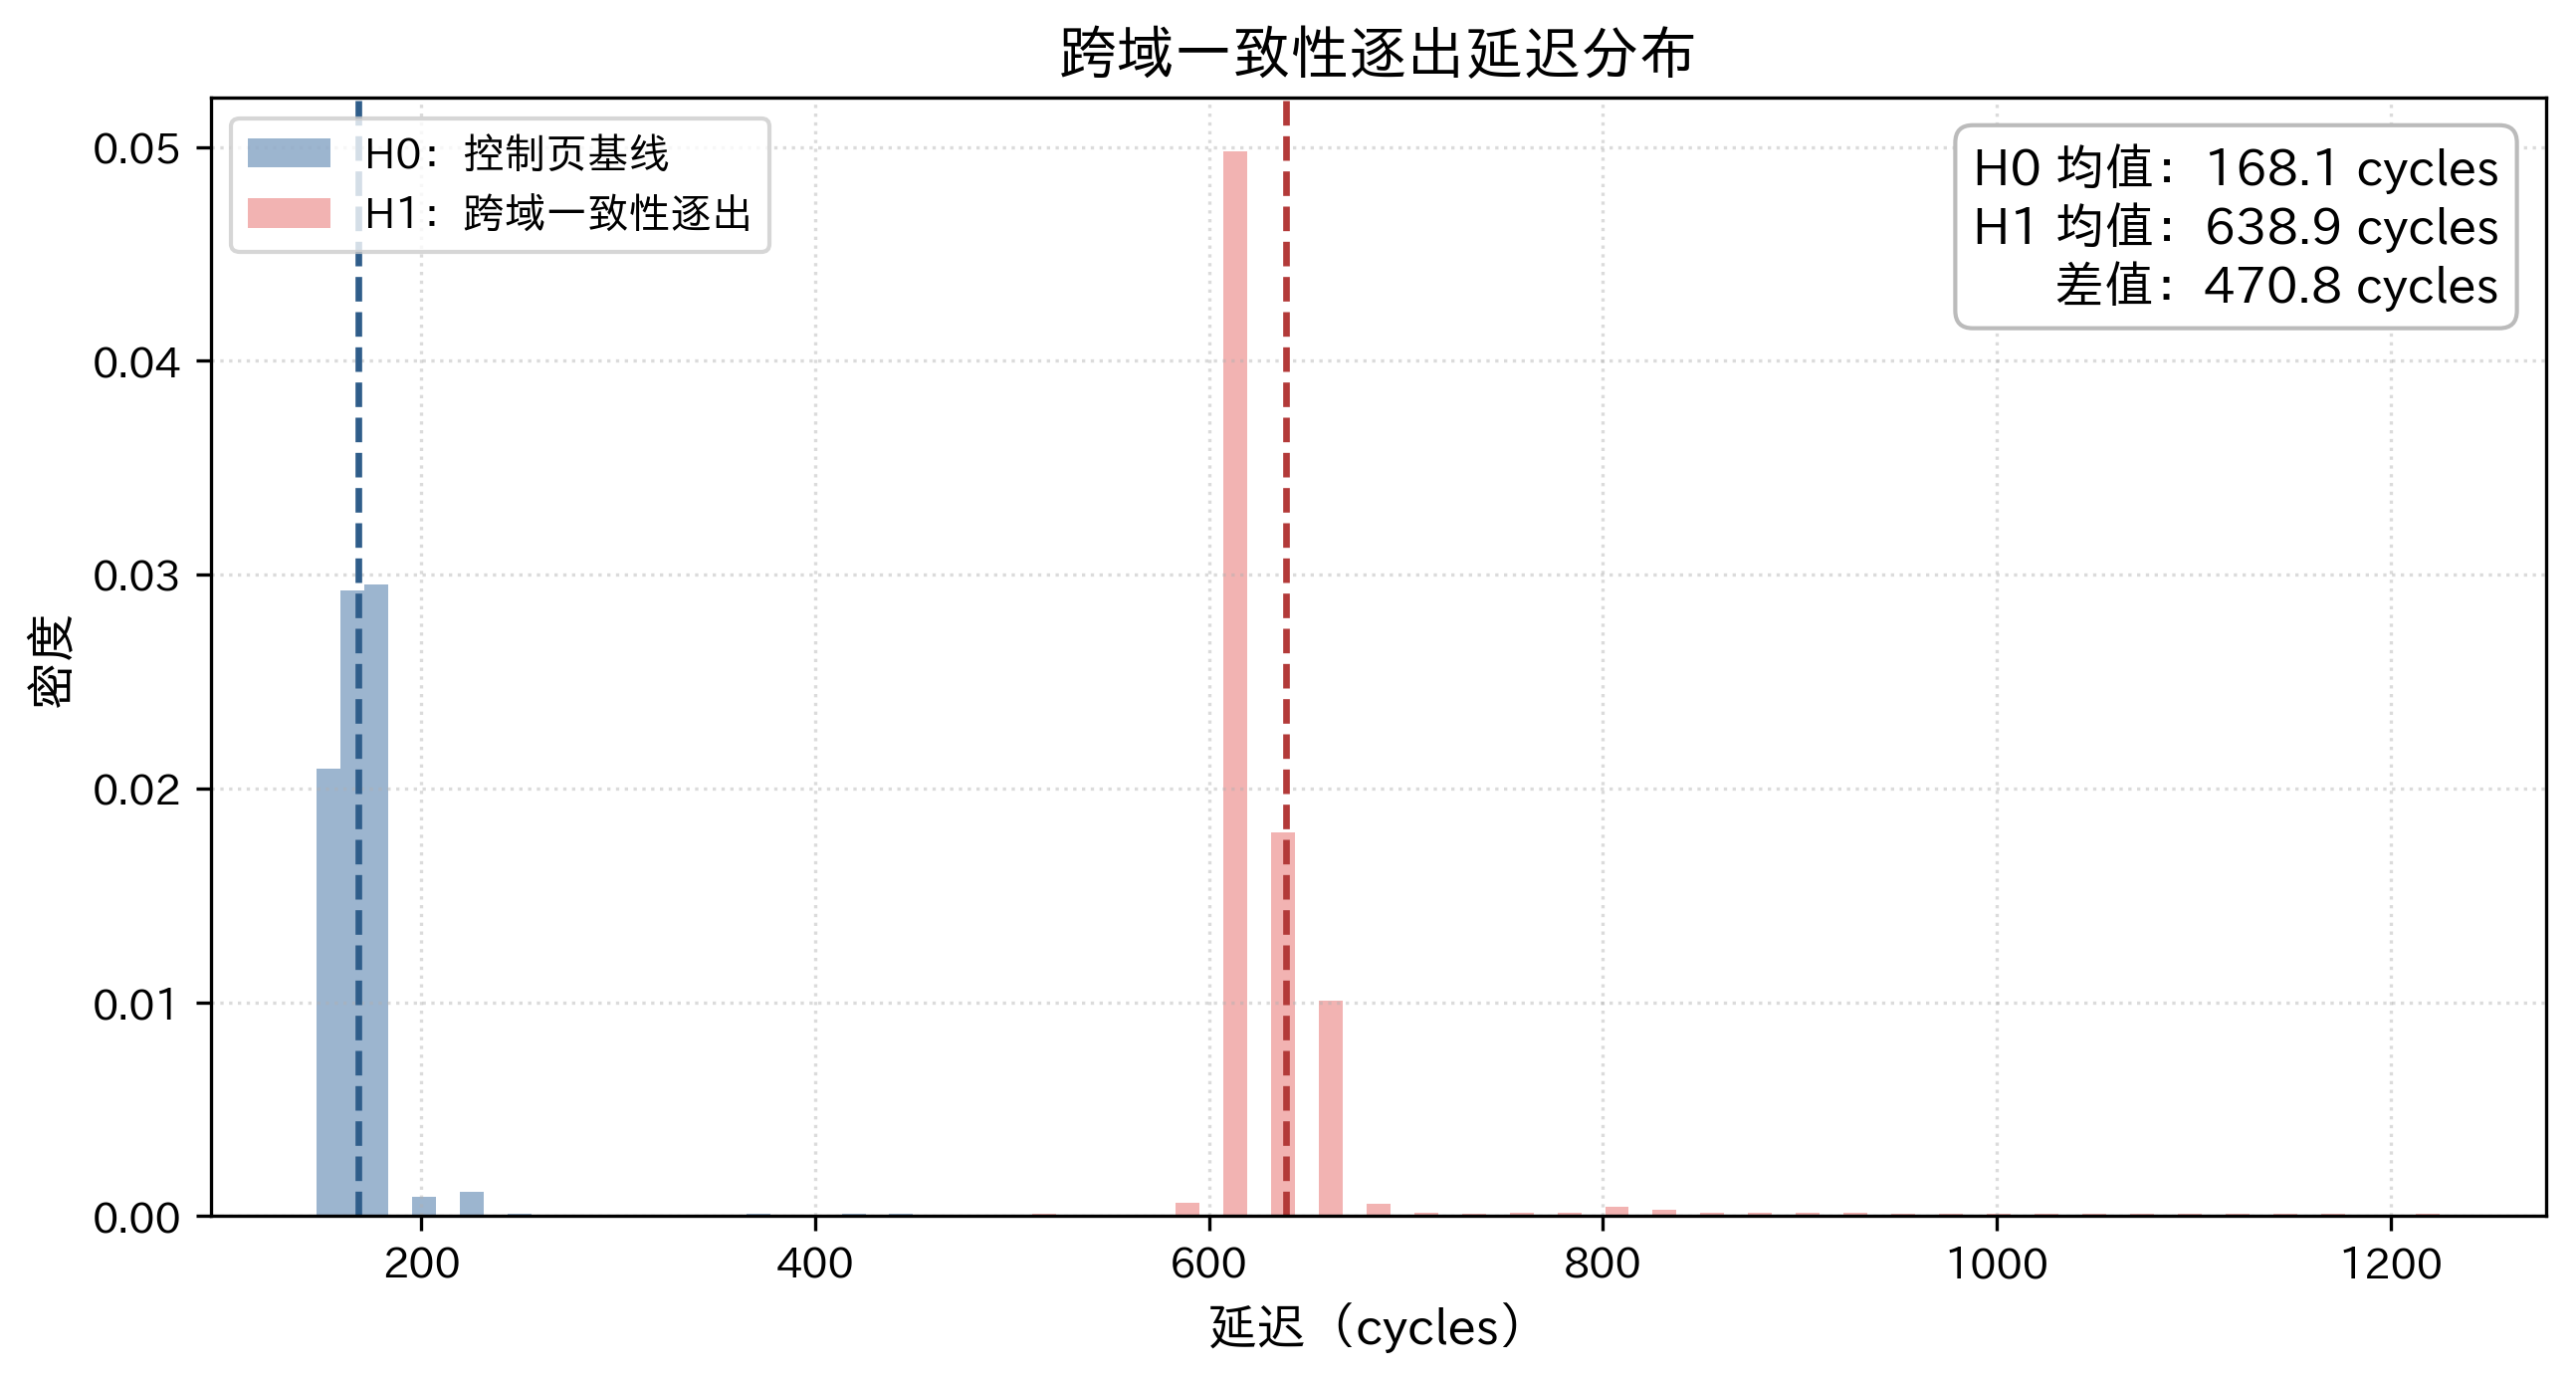
\includegraphics[width=12.2cm]{pic/coherence_42a.png}
  \caption{跨域一致性逐出信号的延迟分布（50000 样本）}
  \label{fig:coherence_42a}
\end{figure}

图~\ref{fig:coherence_42a} 呈现双峰分布，$H_0$ 与 $H_1$ 两组分布核心区间之间无样本重叠。$H_0$ 均值为 73.8 cycles，对应宿主机探测命中本地缓存；$H_1$ 均值为 647.9 cycles，对应缓存逐出后从主存重新加载的开销，两组均值差约为 574 cycles。这一差值本质上是跨域一致性逐出将探测延迟从缓存命中级别（约 70 cycles）抬升至 DRAM 访问级别（约 640 cycles）所形成的，延迟倍数约为 8.7 倍，远超缓存层次间的自然延迟比例，因而易于检测。

$H_1$ 分布形态集中，标准差约为 81 cycles，与两组均值差（574 cycles）相比，分布宽度相对较窄。这意味着判决阈值的选取对误报率的影响不敏感——在 $H_0$ 第 99 百分位与 $H_1$ 第 5 百分位之间存在宽裕的无重叠区间，阈值在该区间内小幅移动不会改变判决结论。对于需要重复多次观测的密钥恢复攻击，这种稳定性使得固定阈值跨实验会话沿用可行，无需对每次攻击单独标定。

\subsection{物理页内的信号空间分布}
\label{subsec:spatial_dist}

本节进一步测量一致性逐出信号在 4KB 物理页内的空间分布情况。图~\ref{fig:heatmap_42aplus} 展示了同页与跨页访问条件下的 64$\times$64 延迟矩阵。

\begin{figure}[htbp]
  \centering
  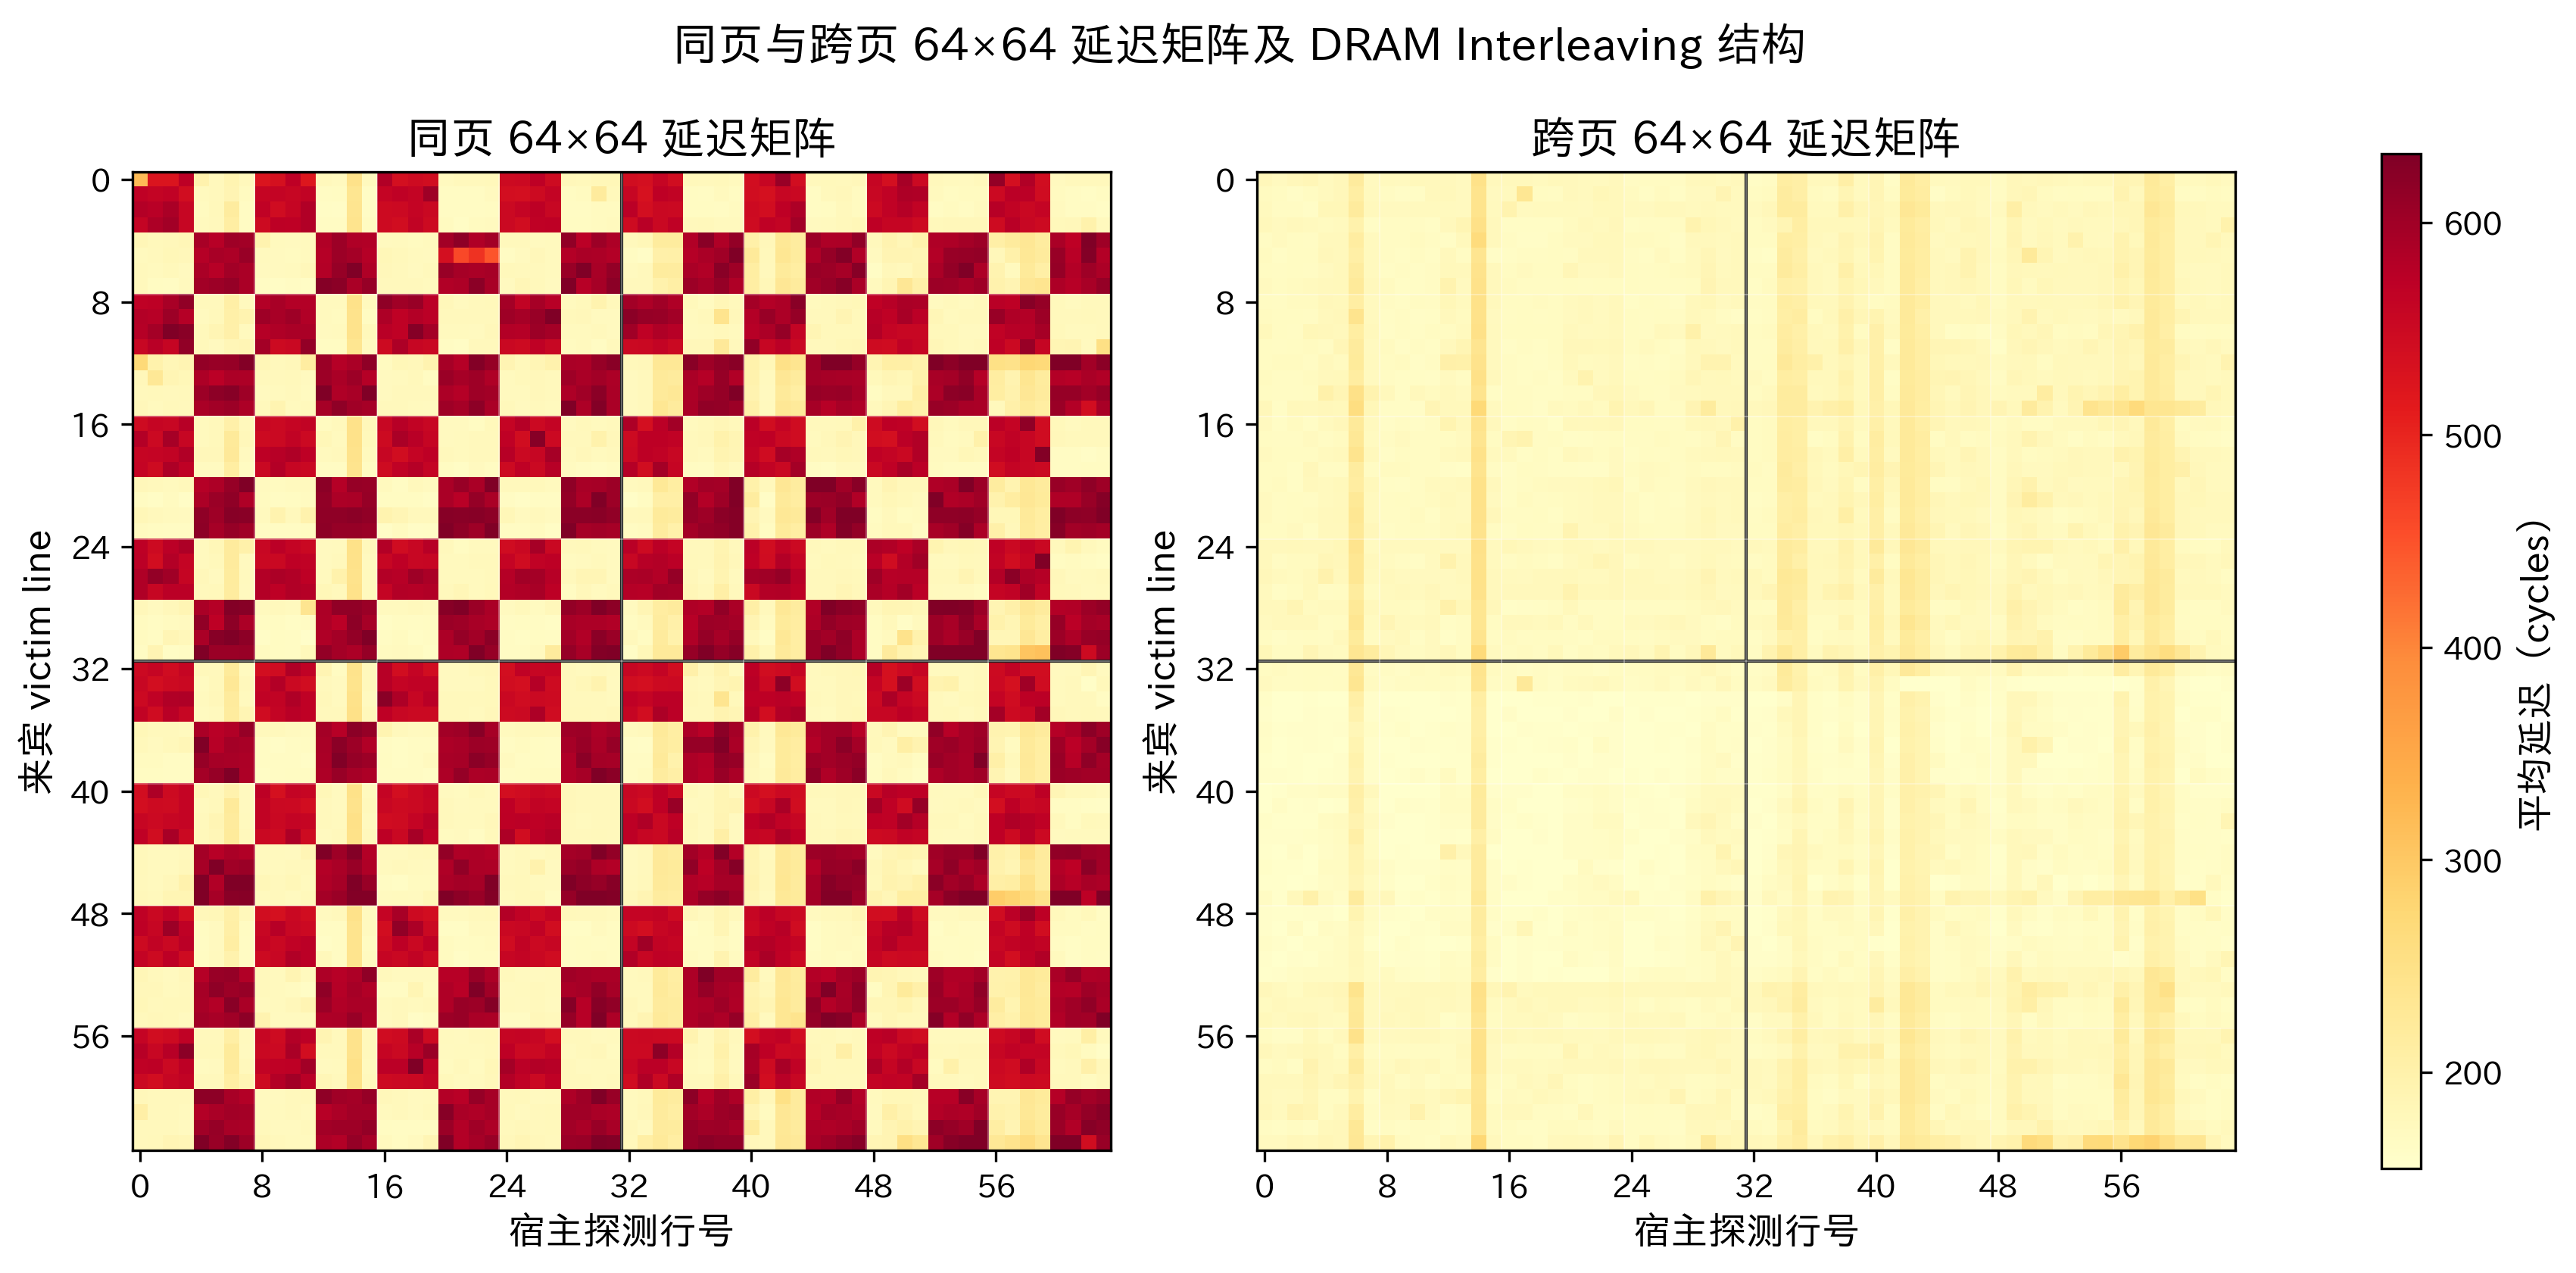
\includegraphics[width=10.8cm]{pic/heatmap_42aplus.png}
  \caption{同页与跨页访问的延迟矩阵热力图}
  \label{fig:heatmap_42aplus}
\end{figure}

图~\ref{fig:heatmap_42aplus} 显示同一物理页内的信号强度分布呈块状和条带结构。这一现象与 DRAM 地址交错机制有关：内存控制器将连续物理地址映射到不同内存通道和 Bank，使物理上相邻的缓存行对应不同的 DRAM 访问路径，延迟因此存在差异。上述分布特征说明页内各位置的信号强度不一致，偏移量为 0 的缓存行不具有代表性。

从热力图的结构来看，信号强度较高的缓存行在页内并非随机分布，而是呈现出与 DRAM 交错块大小相匹配的周期性规律。这说明只要攻击者事先确定目标物理页在 DRAM 中的通道映射关系，即可预测页内哪些缓存行处于强信号区域，而无需对 64 条缓存行逐一测试。对于 AES T-Table 攻击场景，T-Table 在内存中按固定步长对齐存放，其各个缓存行对应的信号强度可以在攻击准备阶段一次性扫描确定，后续多轮观测均复用该信息。

\subsection{物理内存竞争信号测量}

\subsubsection{NOCACHE 路径下的竞争信号测量}

为了单独测量内存竞争信号的强度，本节实验需要排除缓存命中的干扰。宿主机和虚拟机均绕过缓存直接访问主存，强制产生 DRAM 请求。不发生竞争时作为 $H_0$，双方并发访问同一地址时作为 $H_1$，各采集 50000 个样本。

\begin{figure}[htbp]
  \centering
  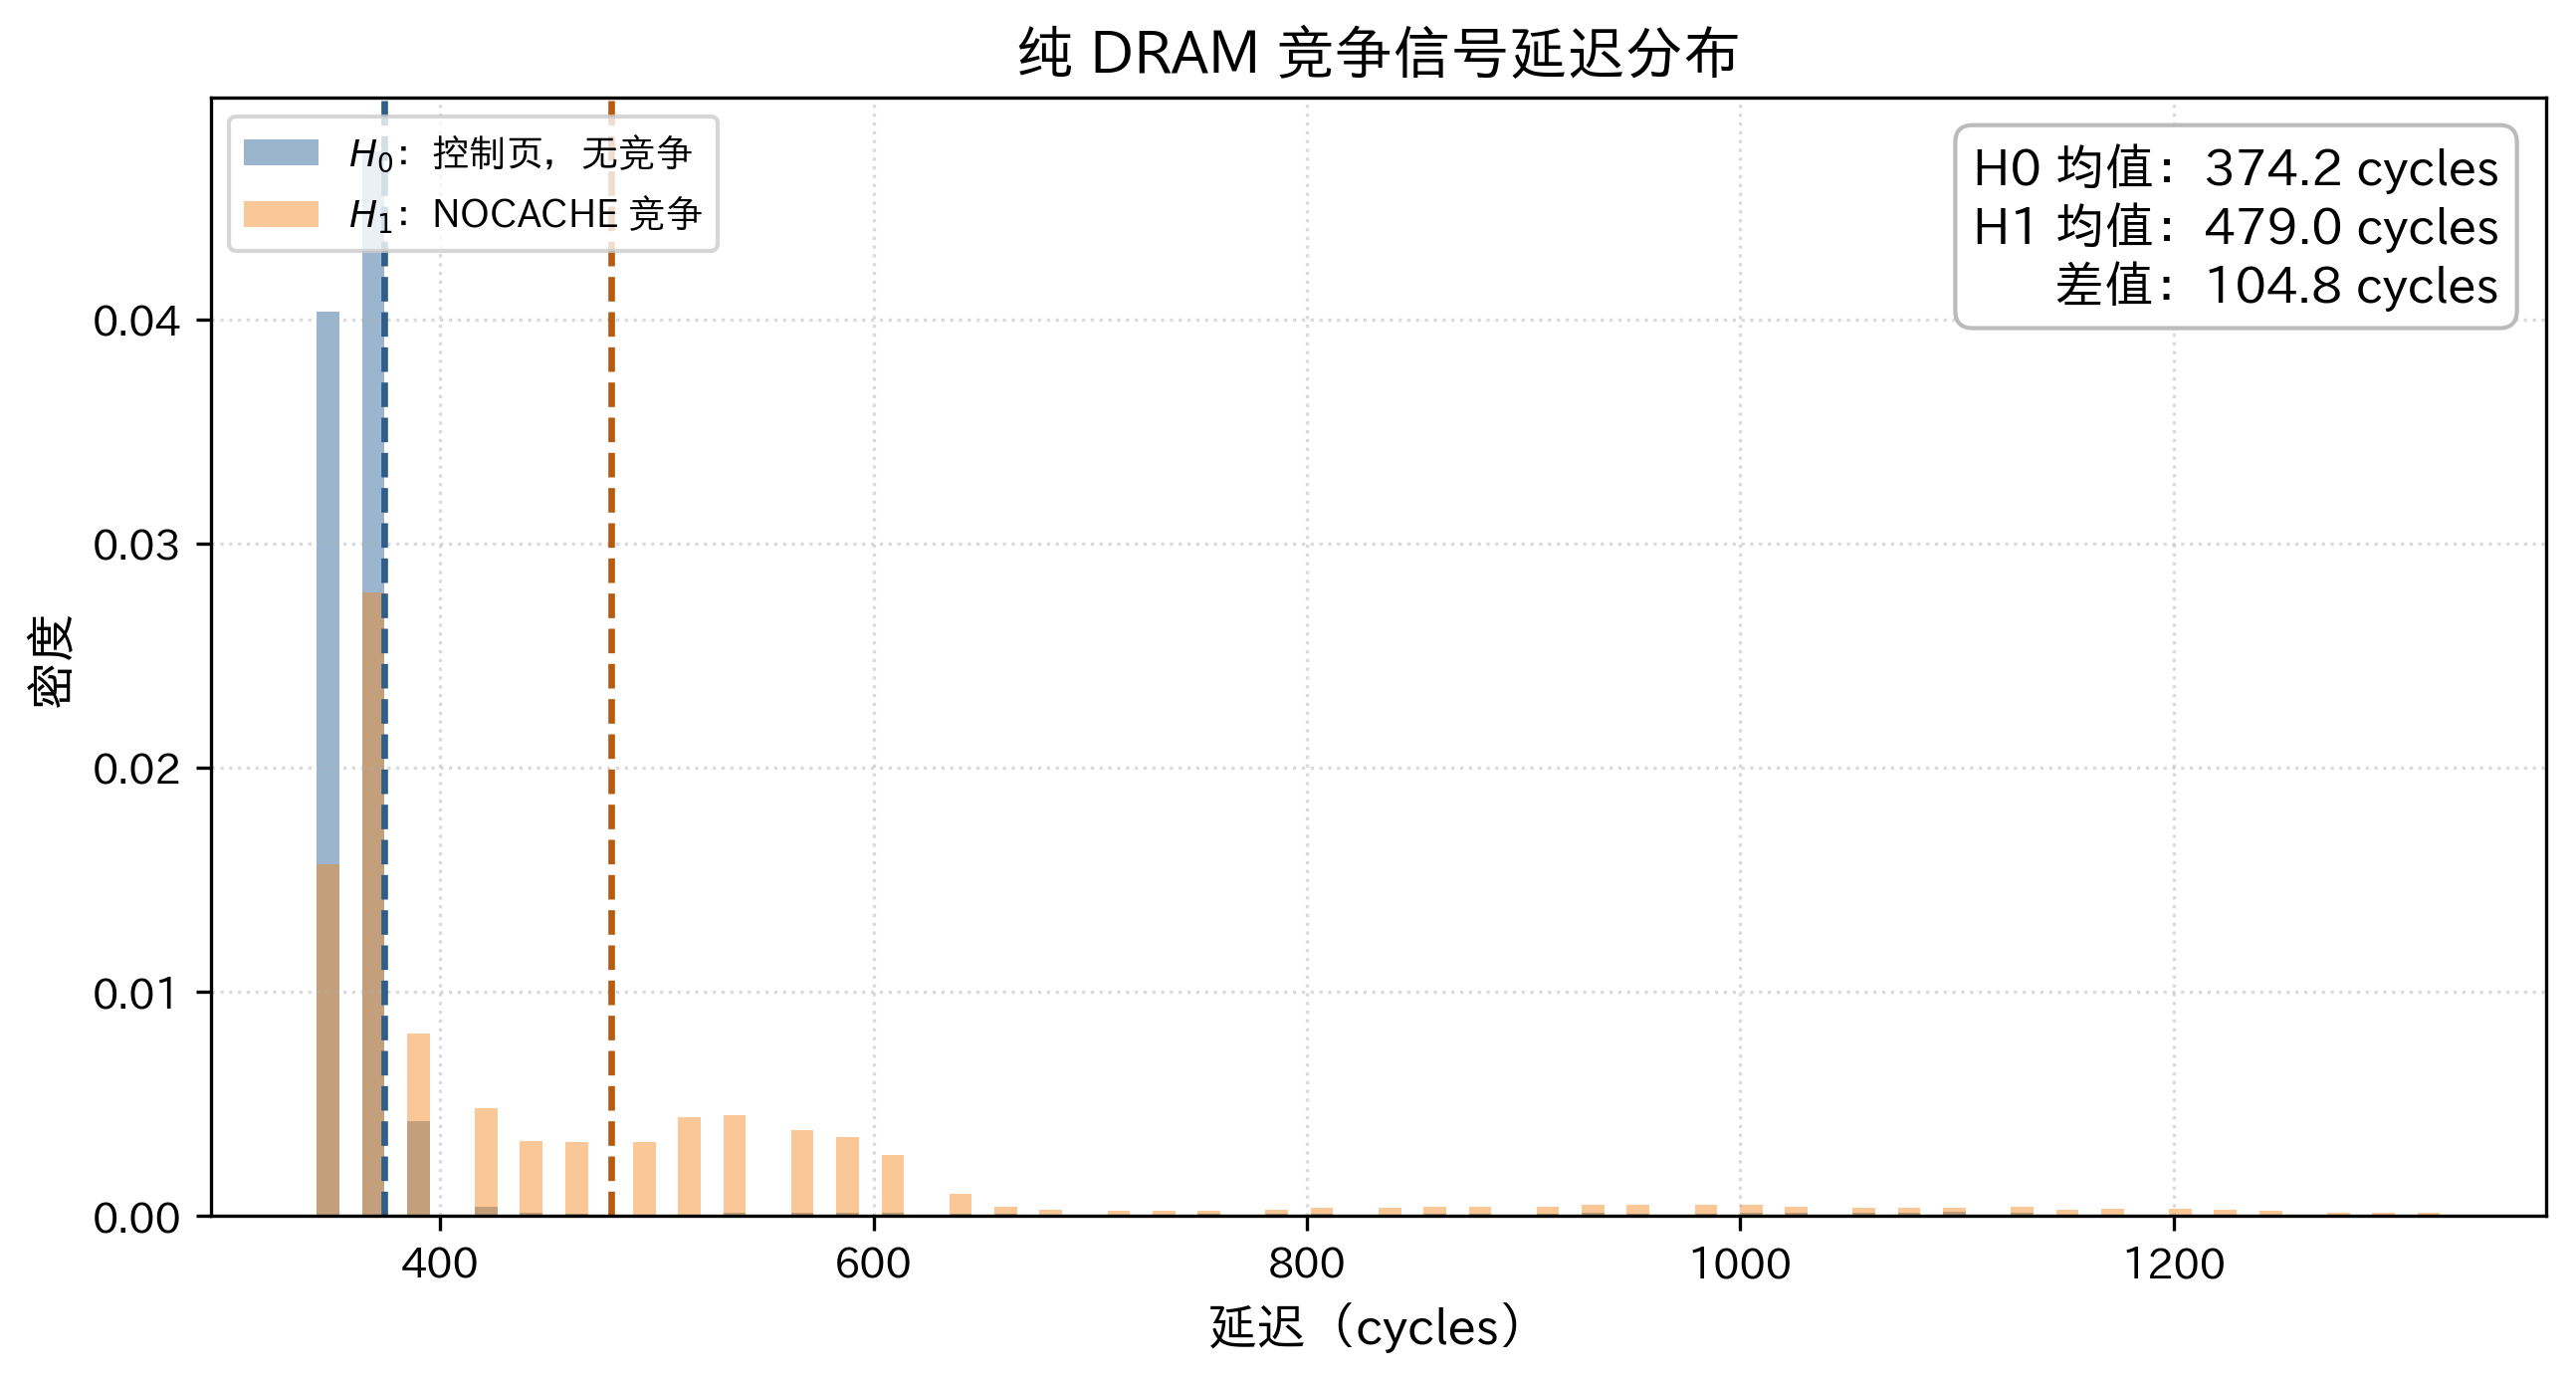
\includegraphics[width=12.2cm]{pic/contention_42b.png}
  \caption{NOCACHE 路径下内存竞争信号的延迟分布（竞争延迟上界）}
  \label{fig:contention_42b}
\end{figure}

两种条件的延迟分布大范围重叠，均值差为 104.8 cycles，$H_1$ 相较于 $H_0$ 主要体现为右尾的延伸。这与一致性逐出信号形成对比：后者呈双峰分布，两组核心区间无重叠；竞争信号则为单峰加尾部的形态，两组分布之间没有清晰边界。这一形态差异揭示了两类机制在触发条件上的本质区别：一致性逐出只要虚拟机访问目标数据即会触发，每次触发均产生可见的延迟跳变；竞争效应则要求双方访问在数十纳秒内精确重叠，多数探测周期内两次访问在时序上存在错位，未能产生有效竞争，因此 $H_1$ 中只有部分样本携带信号，其余样本与 $H_0$ 无法区分。竞争信号不适合用于单次判决，其价值在于与一致性信号结合后提升高置信度判决的比例。

本实验使用 NOCACHE 路径，所测均值差可视为当前硬件上竞争信号强度的参考上界。在实际攻击中，探测路径为 cacheable，需进一步评估。

\subsubsection{Cacheable 路径下竞争信号的独立贡献}

上节实验采用 NOCACHE 路径，两端均绕过缓存直接访问主存，所得结果反映了竞争信号的强度上界。然而在实际攻击场景中，宿主机探测使用的是 cacheable 路径，探测线程维护自身的缓存副本。若宿主机存有热缓存，单次探测直接命中缓存，不产生 DRAM 访问，竞争也就无从发生。因此，在 cacheable 路径下测量竞争信号的独立贡献，需要通过一种方式使宿主机探测强制到达主存，同时不引入一致性逐出信号的干扰。

本实验在每次探测前由宿主机执行 \texttt{CLFLUSH} 指令，将目标缓存行从缓存中清除。清除后探测必须从主存加载数据，同时因缓存中无宿主机副本，不会触发跨域一致性逐出，从而隔离了一致性信号的干扰。来宾侧 $H_1$ 条件下同步执行 \texttt{CLFLUSH} + \texttt{load}，使宿主机和来宾在相近时刻均向同一物理地址发出主存请求，形成 DRAM 总线竞争。两种条件各采集 50000 个样本，延迟分布见图~\ref{fig:contcache_42bb}。

\begin{figure}[htbp]
  \centering
  \includegraphics[width=12.2cm]{pic/contcache_42bb.png}
  \caption{Cacheable 路径竞争信号的延迟分布（50000 样本，CLFLUSH 隔离）}
  \label{fig:contcache_42bb}
\end{figure}

$H_0$ 的基线延迟高于 NOCACHE 路径，原因是 cacheable 路径下的冷加载需经过缓存一致性协议的状态检查，整体开销高于直接绕过缓存的方式。$H_1$ 条件下均值差为 433.7 cycles，高于 NOCACHE 实验的 104.8 cycles，这与来宾 \texttt{CLFLUSH} 操作使两端主存访问的时序对齐程度更高有关——来宾主动将缓存行清除后再 load，使其 DRAM 请求与宿主机的冷加载请求在时序上更可能重叠。

需要注意，这里所测均值差混合了两部分开销：宿主机 \texttt{CLFLUSH} 本身引入的冷加载基础延迟，以及竞争事件叠加的额外延迟。因此，433.7 cycles 不能直接理解为"竞争贡献"，而是在已有 CLFLUSH 冷加载开销基础上的附加延迟。在实际攻击中，宿主机探测通常处于热缓存状态，切换至 CLFLUSH 模式的代价是每次探测都需要一次完整的缓存缺失，这会降低可用的探测频率。$H_1$ 分布形态较宽，强竞争与弱竞争事件均有出现，反映了竞争效应对时序精度的依赖。与一致性逐出信号相比，两组分布重叠程度更高，单次判决的可靠性较低，定量对比见第~\ref{subsec:roc_capacity}节。

\subsubsection{竞争信号的空间定位精度}
\label{subsubsec:contention_spatial}

上述实验在固定物理地址上测量了竞争信号的强度，尚未考察其空间选择性——即当来宾访问某条特定缓存行时，宿主机在同一物理页内其他位置的探测是否也会受到干扰。本实验通过扫描同页内全部 64 条缓存行的探测延迟差，量化竞争信号的空间响应范围。

实验中，来宾在 $H_1$ 条件下以 \texttt{CLFLUSH} + \texttt{load} 持续访问目标页第 32 条缓存行，强制产生 DRAM 级请求。宿主机以 NOCACHE 路径对目标页内编号 0–63 的全部 64 条缓存行逐一扫描，每个位置采集 3000 个样本作为 $H_1$ 延迟；同时以相同偏移量探测一个对照页并采集 3000 个样本作为 $H_0$ 基线，以排除 DRAM 路径本身的延迟波动。两者之差 $\Delta_i = \overline{T}_{H_1,i} - \overline{T}_{H_0,i}$ 反映了该探测位置上竞争效应的净贡献。结果见图~\ref{fig:contention_spatial_42bc}。

\begin{figure}[htbp]
  \centering
  \includegraphics[width=12.2cm]{pic/contention_spatial_42bc.png}
  \caption{物理内存竞争信号的空间响应（固定来宾访问第 32 行，扫描宿主探测位置 0–63）}
  \label{fig:contention_spatial_42bc}
\end{figure}

图~\ref{fig:contention_spatial_42bc} 显示，仅第 32 行的均值差 $\Delta_{32} = 259.7$ cycles 超出背景噪声范围，其余 63 条缓存行的均值差均在噪声水平内，紧邻的第 31 行和第 33 行亦无明显差异。信号选择比约为 14.7，表明竞争信号具有缓存行级别的空间局部性，未见向相邻缓存行扩散的迹象。

上述结果证实了物理内存竞争信号的空间粒度为 64B 缓存行，与其作用机制一致：竞争发生在内存控制器的请求仲裁层面，仅当宿主机与来宾访问同一 64B 物理地址时才会产生信号。14.7 的信号选择比意味着，若宿主机探测的地址偏移了一个缓存行（64B），信号立刻衰减至噪声水平，不存在"部分重叠"的过渡区域。这对攻击者的地址解析精度提出了明确要求：必须获得目标缓存行的精确物理地址（64B 对齐），而非仅知道物理页基址。

这一特性与跨域一致性逐出信号形成互补。一致性信号的逐出粒度由硬件一致性协议决定，本平台为 2KB，详见第~\ref{subsec:spatial_dist}节。一致性信号能可靠检测来宾对目标页的访问，但 2KB 的粒度无法区分页内 32 条缓存行中的具体哪一条被访问；竞争信号的定位精度为 64B，可将范围缩小至单条缓存行。对于 AES T-Table 攻击，每条 64B 缓存行覆盖 16 个 T-Table 条目，对应 16 种密钥字节候选值，竞争信号的缓存行级定位是从 256 个候选值缩小至 16 个所必需的。两类信号在空间精度上的互补关系是第五章两阶段探测设计的实验依据。

\subsection{四路信号对比分析}

本节设计四路对比实验，以统一的 $H_0$ 基线为参照，比较两种信号及其叠加效果。四种测试条件如表~\ref{tab:fourway_design} 所示。

\begin{table}[htbp]
  \centering
  \renewcommand{\arraystretch}{1.2}
  \caption{四路对比实验设计}
  \label{tab:fourway_design}
  \setlength{\tabcolsep}{6pt}
  \begin{tabular}{p{3.2cm}p{3.6cm}p{6.0cm}}
    \hline
    条件 & 宿主探测路径 & 来宾行为 \\
    \hline
    H0（基线）    & cacheable & 不访问目标物理页 \\
    H1 仅一致性   & cacheable，\texttt{sync\_us=200\,\textmu s} & 访问目标缓存行后等待 \\
    H1 仅竞争     & cacheable + 预先 \texttt{CLFLUSH} & 并发执行 \texttt{CLFLUSH} + \texttt{load} \\
    H1 一致性+竞争 & cacheable，无同步等待 & 与宿主探测并发访问目标缓存行 \\
    \hline
  \end{tabular}
\end{table}

仅竞争条件下，宿主机预先清空目标缓存行，以排除一致性信号的干扰。一致性+竞争条件下，去掉同步等待，使虚拟机与宿主机的访问时间尽量重叠，令两种信号同时产生。各测试条件的采样规模有所不同：基线与仅一致性条件各采集 50000 个样本，仅竞争与叠加条件各采集 20000 个样本，结果记录在表~\ref{tab:stats_fourway} 中。

\begin{figure}[htbp]
  \centering
  \includegraphics[width=12.2cm]{pic/fourway_42c.png}
  \caption{四路条件下的延迟分布对比}
  \label{fig:fourway_42c}
\end{figure}

\begin{table}[htbp]
  \centering
  \renewcommand{\arraystretch}{1.2}
  \caption{四路条件统计量对比}
  \label{tab:stats_fourway}
  \begin{tabular}{lccccc}
    \hline
    条件 & 均值（cyc）& 中位数（cyc）& 标准差（cyc）& $P(T>700)$ & $P(T>1000)$ \\
    \hline
    H0 基线         & 73.8 & 73 & 165.1$^\dagger$ & 0.01\%     & 0.01\% \\
    H1 仅一致性     & 647.9 & 637 & 347.8$^\dagger$ & 2.53\% & 1.10\% \\
    H1 仅竞争       & 949.3 & 1029 & 430.2 & 71.07\% & 57.89\% \\
    H1 一致性+竞争  & 823.9 & 735 & 467.0 & 62.44\% & 30.83\% \\
    \hline
    \multicolumn{6}{l}{\footnotesize $^\dagger$该组含少量调度中断离群值；去除首尾各 1\% 后的标准差分别约为 5.7 和 30.6 cycles} \\
  \end{tabular}
\end{table}

仅一致性条件的延迟分布与 $H_0$ 之间存在较大间隔，详细统计量见表~\ref{tab:stats_fourway}。仅竞争条件因宿主机预先执行 \texttt{CLFLUSH}，基础延迟包含冷加载开销，与其他条件的测量起点不同，绝对延迟不宜直接进行比较。

一致性+竞争条件与仅一致性相比，均值有所上升，但更明显的变化体现在高延迟尾部：$P(T>700)$ 从 2.53\% 上升至 62.44\%，$P(T>1000)$ 从 1.10\% 上升至 30.83\%。两类信号叠加时，竞争效应并非均匀增加延迟，而是主要扩大极端高延迟事件的发生概率。从机制上看，一致性逐出决定探测是否能捕获来宾访问，竞争效应则在此基础上进一步增大高延迟样本的比例，提高判决置信度。这与第三章对两类机制时序窗口的分析相符。

\subsection{ROC 曲线与物理信道容量}
\label{subsec:roc_capacity}

本节对两类信号的判决准确性进行定量分析，确定各自的最优判决阈值，并从信息论角度估算信道容量。

在第三章建立的 $H_0/H_1$ 二元假设检验框架（式~\ref{eq:threshold_detect}）中，攻击者以固定阈值 $\theta$ 对每次探测延迟进行判决：延迟超过 $\theta$ 则判定受害者访问了目标（$H_1$），否则判定未访问（$H_0$）。阈值的选取面临权衡——$\theta$ 降低时检测率 $P_D$ 升高，同时误报率 $P_{FA}$ 也随之上升。接收者操作特征（Receiver Operating Characteristic，ROC）曲线遍历所有可能的阈值，将对应的 $(P_{FA},\,P_D)$ 点连成一条曲线，直观展示两类误差之间的全局权衡关系。曲线越靠近左上角，信号整体可区分性越好；对角线（$P_D = P_{FA}$）对应随机猜测。ROC 曲线下面积（Area Under the Curve，AUC）给出了一个汇总指标：它等于随机抽取一个 $H_1$ 样本的延迟大于随机抽取一个 $H_0$ 样本延迟的概率——AUC = 1 表示两组分布完全可分，AUC = 0.5 表示无区分能力。最优判决阈值 $\theta^*$ 由 Youden's J 指数（$J = P_D - P_{FA}$）最大化确定，在检测率与误报率之间取最佳平衡点。

信道容量以"比特/次探测"为单位，衡量单次探测可传递的最大侧信道信息量。本文将该二元侧信道建模为二元非对称信道（Binary Asymmetric Channel，BAC），信道的前向概率为 $P_D$（输入 $H_1$ 时输出 $H_1$ 的概率）和 $P_{FA}$（输入 $H_0$ 时输出 $H_1$ 的概率），其容量为
\begin{equation}
  C = \max_{p \in [0,1]} \left[ H_b\!\left(p P_D + (1-p) P_{FA}\right) - p\,H_b(P_D) - (1-p)\,H_b(P_{FA}) \right],
  \label{eq:bac_capacity}
\end{equation}
其中 $H_b(p) = -p\log_2 p - (1-p)\log_2(1-p)$ 为二元熵函数，$p$ 为 $H_1$ 的先验概率，对 $p$ 的优化给出信道容量的上界。信道容量乘以探测频率即为理论侧信道带宽。

\begin{figure}[htbp]
  \centering
  \includegraphics[width=13.6cm]{pic/roc_42de.png}
  \caption{两类侧信道信号的 ROC 曲线（左：跨域一致性逐出；右：物理内存竞争）}
  \label{fig:roc_42de}
\end{figure}

图~\ref{fig:roc_42de} 展示了两类信号各自的 ROC 曲线。

跨域一致性逐出信号在最优阈值处的检测率 $P_D = 1.0000$，误报率 $P_{FA} = 0.0001$，对应信道容量为 0.9993 比特/次探测。$P_{FA}$ 的极小值来自少量调度中断引起的 $H_0$ 离群值，两组核心分布无重叠。AUC 为 0.9351，受少量极端离群值影响，低于工作点附近的实际可区分度。从密钥恢复的角度看，$P_{FA} \approx 0.0001$ 意味着每万次探测中仅有约 1 次误报，误报对相关性分析的污染极低；$P_D \approx 1.0$ 则保证了来宾每次目标访问几乎都能被捕获，不会因漏检而丢失信息。这两个特性共同决定了极少量的探测轮次即可建立可靠的统计相关。

物理内存竞争信号在最优阈值处的检测率 $P_D = 0.8709$，误报率 $P_{FA} = 0.0552$，信道容量为 0.5652 比特/次探测，AUC 为 0.9007。$P_{FA}$ 约为一致性信号的 550 倍，反映出两组分布重叠程度较高。这一差异源于竞争效应对时序精度的依赖：信号仅在两端 DRAM 访问在纳秒级时间窗口内重叠时出现，随机性较强，分布较分散。若单独依赖竞争信号进行密钥恢复，较高的 $P_{FA}$ 会向相关性分析中引入较多噪声，需要更多重复观测才能收敛至正确密钥字节；而与一致性信号配合使用时，一致性信号先提供可靠的"是否访问"判决，竞争信号再提供高精度的缓存行定位，两者分工可以将各自的误差控制在可接受范围内。

\begin{figure}[htbp]
  \centering
  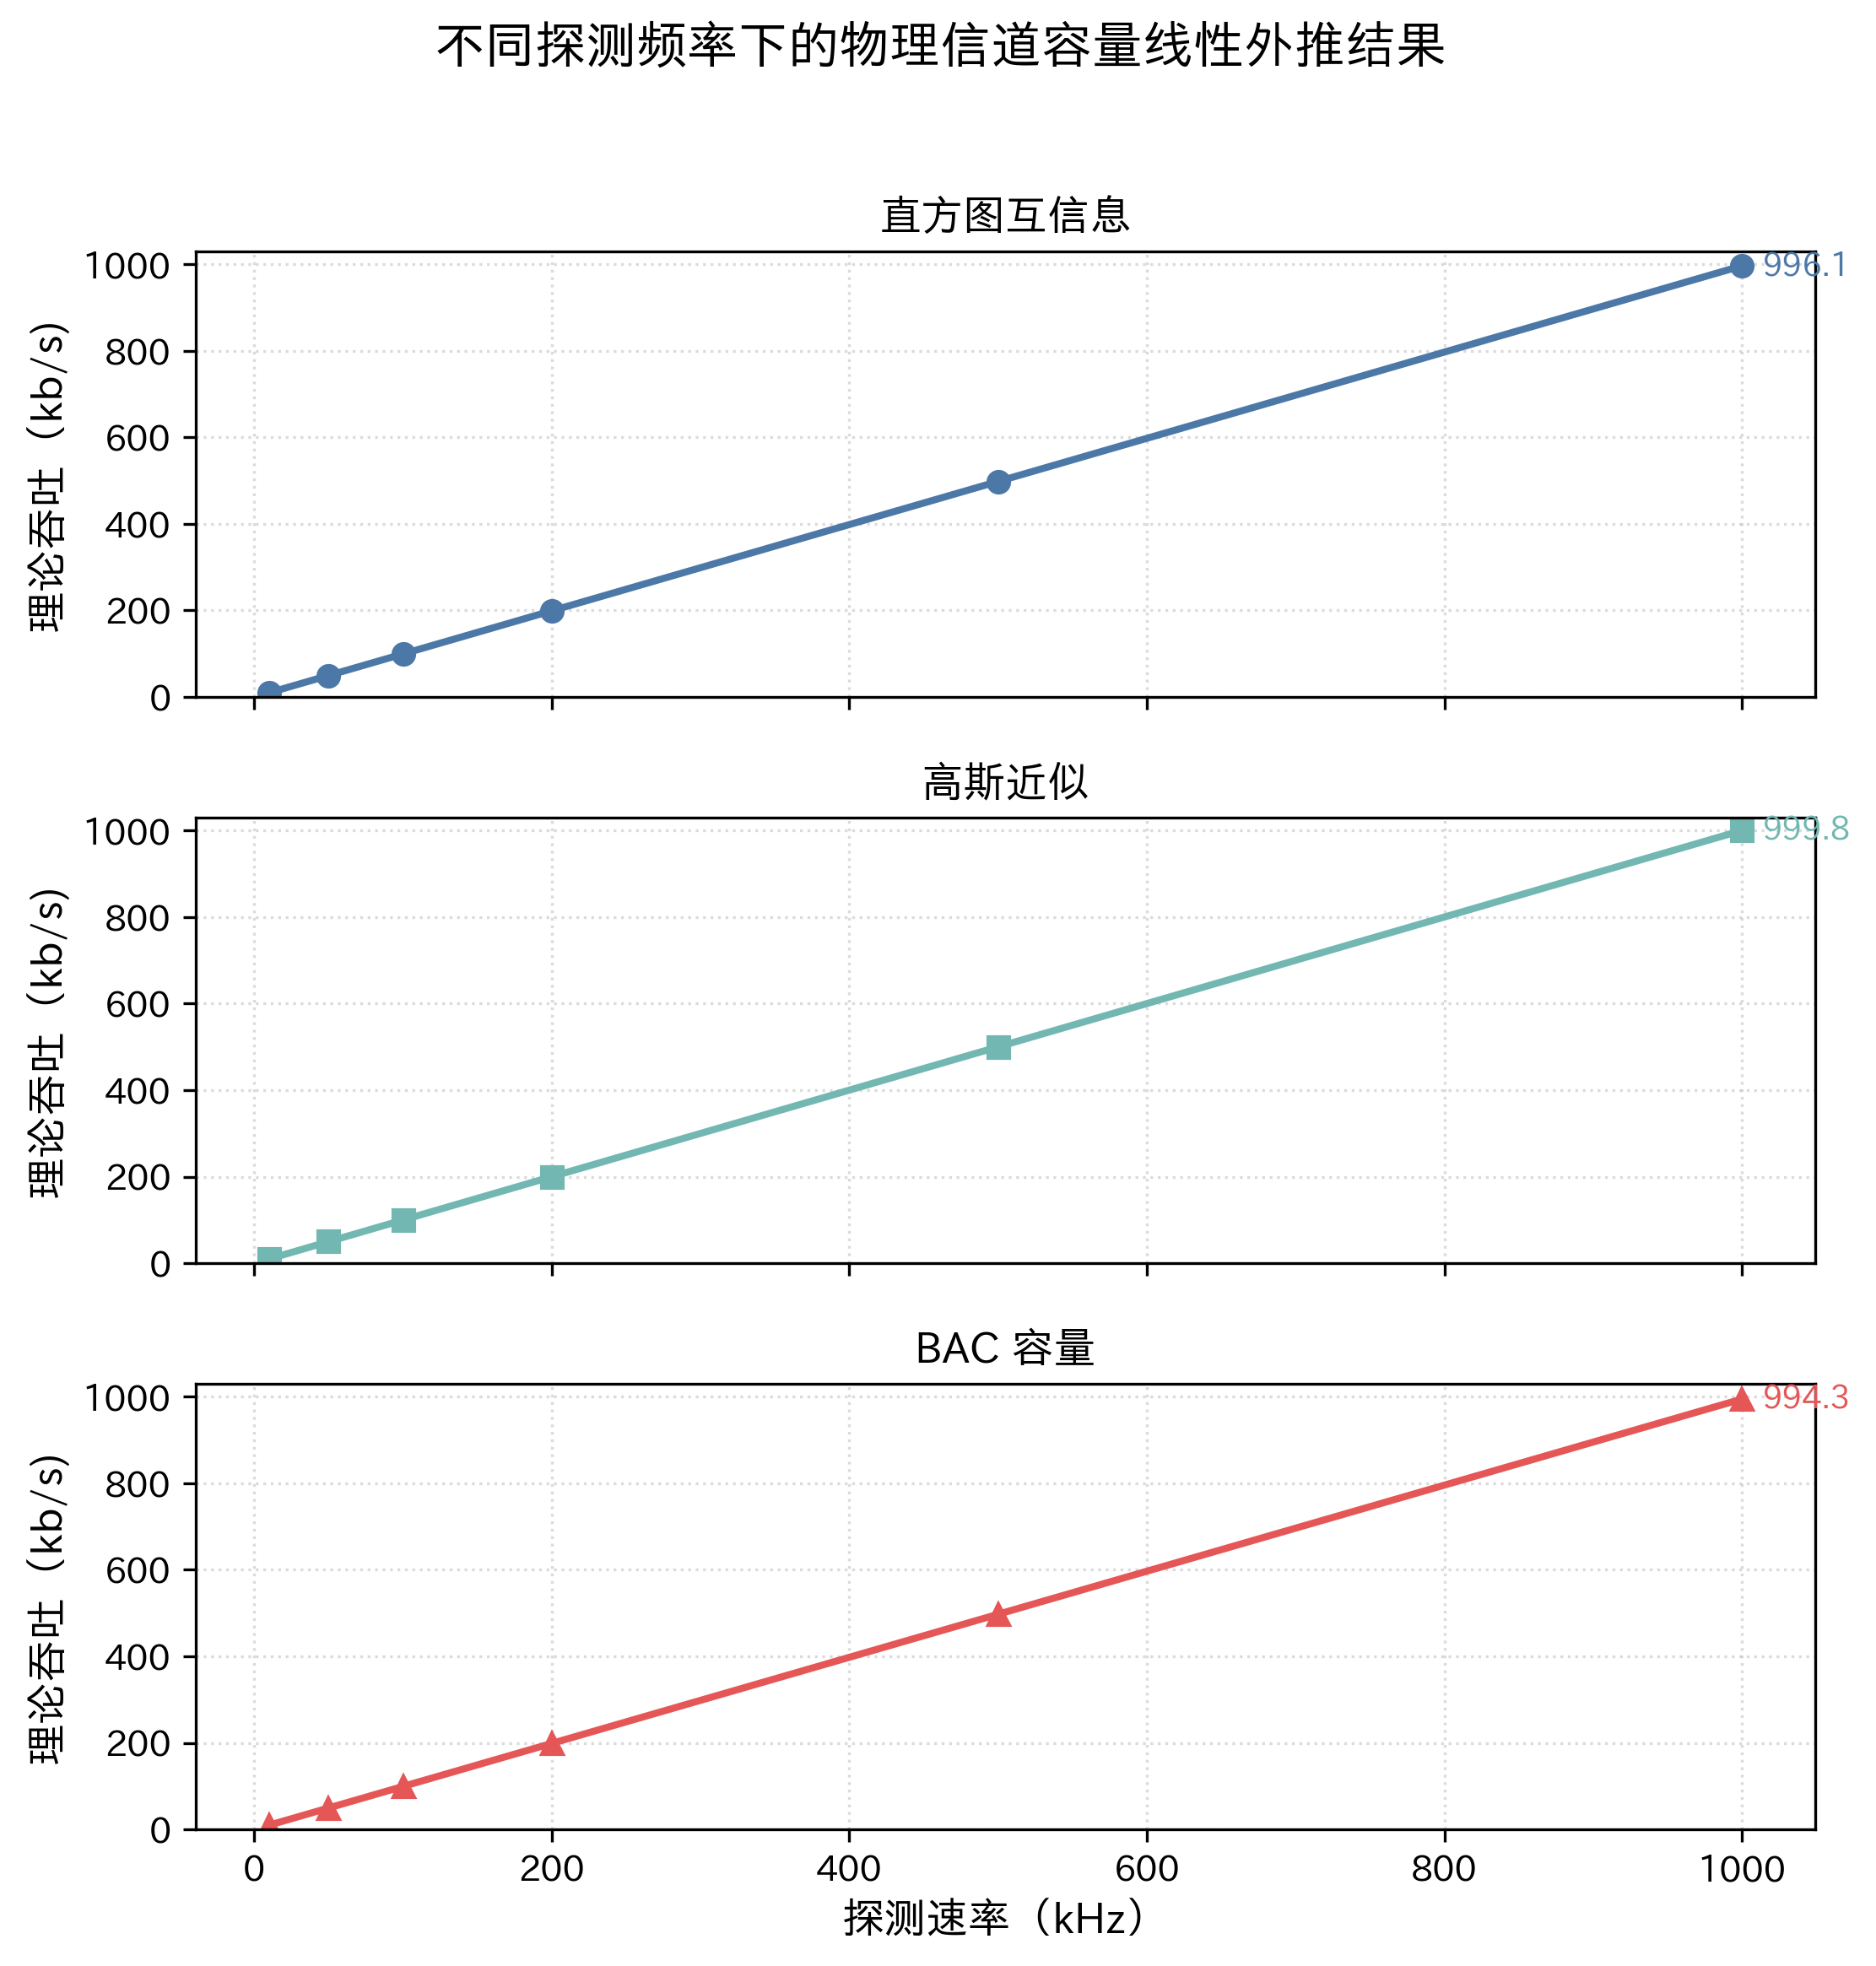
\includegraphics[width=10.4cm]{pic/capacity_42e.png}
  \caption{不同探测频率下一致性逐出信号的物理信道容量推算结果}
  \label{fig:capacity_42e}
\end{figure}

图~\ref{fig:capacity_42e} 给出了一致性逐出信号在不同探测频率下的理论信道吞吐率。对于 128 比特 AES 密钥恢复任务，两类信号的信道容量本身不构成主要限制，实际攻击中的瓶颈更多来自同步精度、系统噪声以及密钥推断算法的效率，这些问题将在第五章讨论。

\section{系统噪声对信号的影响}

前面的实验在受控环境下进行，排除了系统级干扰。在真实的云环境中，并发负载、操作系统线程调度和硬件中断会改变延迟分布，进而影响固定阈值的判决效果。本节测试多进程负载与线程调度、中断对信号强度的影响。

\subsection{系统负载对信号的影响}

一致性信号依赖探测线程与 vCPU 共享 L1/L2 缓存，处理器调度行为对信号质量有直接影响。表~\ref{tab:noise_load_43a} 给出了四种系统负载条件下的信号统计量。

\begin{table}[htbp]
  \centering
  \renewcommand{\arraystretch}{1.2}
  \caption{不同系统负载下的一致性信号统计量}
  \label{tab:noise_load_43a}
  \setlength{\tabcolsep}{6pt}
  \begin{tabular}{lcccccc}
    \hline
    条件 & H0 均值 & H0 标准差 & H1 均值 & H1 标准差 & SNR & AUC \\
    \hline
    空载 & 85.6671 & 27.7244 & 515.0060 & 80.9754 & 7.0940 & 0.9977 \\
    CPU 满载 & 99.0822 & 20.6777 & 429.5823 & 196.3446 & 2.3674 & 0.8044 \\
    内存带宽压力 & 83.4819 & 21.4570 & 513.5466 & 80.7315 & 7.2809 & 0.9949 \\
    多 VM 并发 & 83.4665 & 20.4397 & 519.8393 & 88.4282 & 6.7995 & 0.9965 \\
    \hline
  \end{tabular}
\end{table}

CPU 满载对信号质量的影响明显高于其他负载条件，AUC 从 0.99 降至 0.80。满载时操作系统的线程抢占和迁移会使探测线程与 vCPU 分离，两者不再共享 L1/L2 缓存，导致 $H_1$ 分布标准差显著增大。内存带宽压力和多 VM 并发两种负载主要增加内存总线压力，对核间缓存共享关系影响有限，信号质量变化不明显。

内存带宽压力不影响信号质量这一结果值得关注。跨域一致性逐出的关键延迟路径是 L1/L2 缓存状态的跨域失效，而非 DRAM 读取带宽本身；即便内存总线已有较高负载，只要探测线程与 vCPU 共享缓存的拓扑关系保持不变，信号就能稳定产生。这说明该侧信道信号对共存租户的内存访问行为具有较强的鲁棒性，在多租户云环境中不容易因背景流量干扰而失效。探测线程与 vCPU 的核间绑定是维持信号稳定性的关键条件，也是攻击部署时需要首先满足的硬性前提。

\subsection{中断与调度抖动的影响}

本节测试线程调度和硬件中断对延迟稳定性的影响，对比绑核隔离与不绑核两种情况，结果见表~\ref{tab:sched_jitter_43b}。

\begin{table}[htbp]
  \centering
  \renewcommand{\arraystretch}{1.2}
  \caption{绑核与不绑核条件下的调度抖动统计}
  \label{tab:sched_jitter_43b}
  \setlength{\tabcolsep}{6pt}
  \begin{tabular}{lcccccc}
    \hline
    条件 & H0 均值 & H0 标准差 & H1 均值 & H1 标准差 & H0 3$\sigma$ 比例 & H1 3$\sigma$ 比例 \\
    \hline
    绑核 + 隔离核心 & 114.4873 & 28.5649 & 596.6552 & 63.9406 & 1.8\% & 1.9\% \\
    不绑核 & 111.9246 & 15.1471 & 628.2902 & 74.8914 & 0.1\% & 2.4\% \\
    \hline
  \end{tabular}
\end{table}

绑核条件下，硬件中断若落在被绑定的核心上，处理时间会直接叠加到探测延迟，使 $H_0$ 的 3-sigma 离群比例高于不绑核。不绑核时 \texttt{irqbalance} 将中断分散到多个核心，$H_0$ 延迟相对平稳，但线程迁移使部分 $H_1$ 样本延迟偏低，$H_1$ 稳定性下降。

从密钥恢复攻击的角度分析，$H_0$ 离群值和 $H_1$ 漏检对攻击效果的影响不对称。$H_0$ 离群值产生的误报会向相关性分析引入少量噪声，但离群值的出现率相对固定且可通过调高判决阈值进一步抑制，对最终收敛的影响有限。$H_1$ 漏检则意味着来宾的真实访问事件被错误标记为"未访问"，直接导致密钥字节与观测序列的相关性降低，需要通过增加观测轮次来弥补，代价更高。因此，绑核方案以可预期的 $H_0$ 离群值换取 $H_1$ 的稳定检测，对攻击整体而言是合理的取舍。

% \subsection{DRAM 地址交错对定位精度的影响}

% 本节分析空间维度上的干扰。DRAM 地址交错机制使同一物理页内相邻缓存行的访问延迟存在差异，本节量化这种机制对定位精度的影响。

% 实验将一个 4KB 页面按不同粒度分成若干组，以探测延迟最高的一组作为预测结果。若虚拟机实际访问的缓存行在该组内，则记为定位正确。实验测试了四种分组大小，结果见表~\ref{tab:granularity_43d}。

% \begin{table}[htbp]
%   \centering
%   \renewcommand{\arraystretch}{1.2}
%   \caption{不同粒度下的定位准确率}
%   \label{tab:granularity_43d}
%   \setlength{\tabcolsep}{6pt}
%   \begin{tabular}{lccc}
%     \hline
%     粒度 & 分组方式 & 组数 & 定位准确率 \\
%     \hline
%     64B 缓存行 & 连续分组 & 64 & 0.109375 \\
%     256B 块 & 连续分组 & 16 & 0.187500 \\
%     1/4 页 & 页内聚合 & 4 & 0.734375 \\
%     1/2 页 & 页内聚合 & 2 & 1.000000 \\
%     \hline
%   \end{tabular}
% \end{table}

% 表~\ref{tab:granularity_43d} 的结果显示，定位准确率与分组粒度并非单调正比关系。按 64B 和 256B 细粒度划分时，准确率较低，这与地址交错机制的作用一致：信号被分散到不同内存通道，延迟最高的单个缓存行不一定是虚拟机实际访问的那条。粒度扩大至 1/4 页和 1/2 页时，准确率明显提升，这种大块划分更有可能将同一内存通道的地址聚合在一起，使分组内的信号响应趋于一致。当分组大小与本平台的交错粒度（1/2 页，即 2\,KB）匹配时，定位准确率达到 100\%。上述结果表明，在不了解目标平台 DRAM 交错参数的情况下，按最细粒度进行监听存在较大的误判风险，预先扫描或根据平台参数确定合适的监听粒度有助于提高定位可靠性。

% 为了进一步观察交错机制的影响，本节还设计了逐出矩阵实验。实验遍历虚拟机访问位置和宿主机探测位置的所有组合，记录不同交错大小（interleaving size）设置下的延迟差。数据汇总在表~\ref{tab:interleaving_43e}中。

% % TODO: 4.3-E 数据补测中，后续补入逐出矩阵图与表~\ref{tab:interleaving_43e} 的定量结果。

% \begin{table}[htbp]
%   \centering
%   \renewcommand{\arraystretch}{1.2}
%   \caption{不同 Interleaving size 下两类信号的统计对比（待补充）}
%   \label{tab:interleaving_43e}
%   \setlength{\tabcolsep}{6pt}
%   \begin{tabular}{lccc}
%     \hline
%     Interleaving size & 一致性信号 $\Delta$（cyc）& 竞争信号 $\Delta$（cyc）& 备注 \\
%     \hline
%     256B  & \todo{补充} & \todo{补充} & \\
%     512B  & \todo{补充} & \todo{补充} & \\
%     1024B & \todo{补充} & \todo{补充} & \\
%     2048B & \todo{补充} & \todo{补充} & \\
%     \hline
%   \end{tabular}
% \end{table}
